% =====================================================================
% Slide 7: Stage 1 -- random alloy generator
% =====================================================================
\begin{frame}{Stage 1: Alloy Configuration Generation}
\fwtag{Python / NumPy}
\begin{columns}[T]
\column{0.42\textwidth}
\textbf{Sampling.}\\
Uniform draws on the 12-element composition simplex\\
(Al, Co, Cr, Cu, Fe, Mg, Mn, Mo, Ni, Si, Ti, Zn);\\
Al-weighted to oversample the aluminium-alloy region.

\bigskip
\textbf{Corpus statistics.}\\
\textbf{7879} configurations generated;\\[0.15em]
\textbf{7815 retained} after the physicality filter\\
\scriptsize ($0 < E < 400$\,GPa,\ $0 < \nu < 0.5$).

\column{0.57\textwidth}
\centering
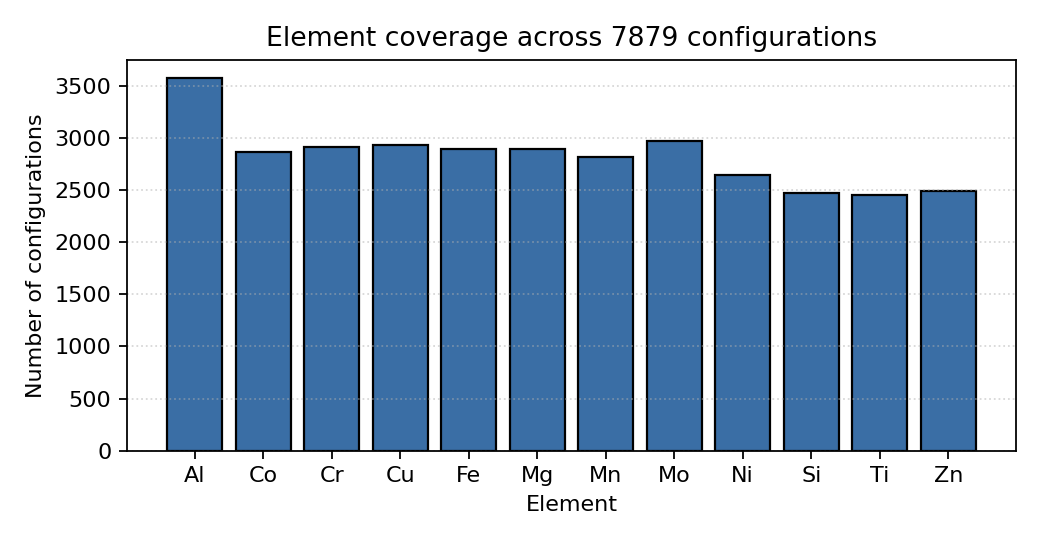
\includegraphics[width=0.98\linewidth]{figures/element_frequency.png}\\[-0.2em]
\scriptsize Element-occurrence distribution over the full
generated corpus.
\end{columns}
\end{frame}
